\section{Auswertung}
\label{sec:Auswertung}

\begin{table}
  \centering
  %\caption{Messwerte x und y sowie das Ergebnis nach Gleichung blabla.}
  \csvreader[tabular=c|c|c,
  head=false, 
  table head= $I\:/\:\si{\ampere}$ & $B\:/\:\si{\milli\tesla}$ & $H \:/\: \si{\ampere}$ \\\midrule,
  late after line= \\]
  {tabelle1.csv}{1=\eins, 2=\zwei, 3=\drei}{$\num{\eins}$ & $\num{\zwei}$ & $\num{\drei}$}
  \label{tab:messwerte}
\end{table}
\begin{figure}
  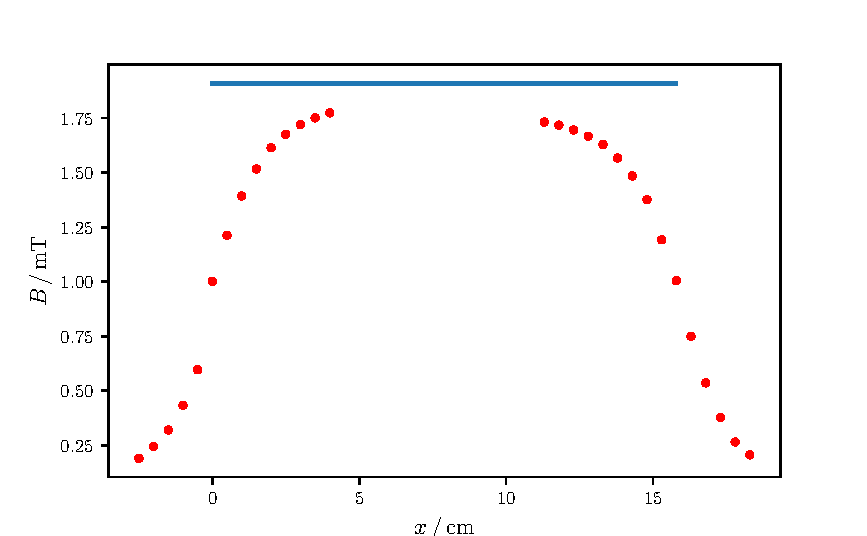
\includegraphics{plot1-1.pdf}
\end{figure}
\begin{figure}
  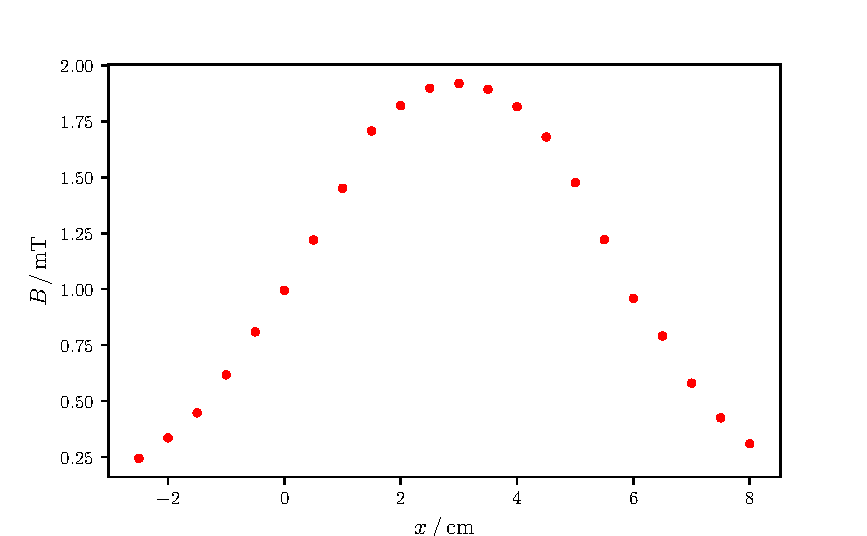
\includegraphics{plot1-2.pdf}
\end{figure}
\begin{figure}
  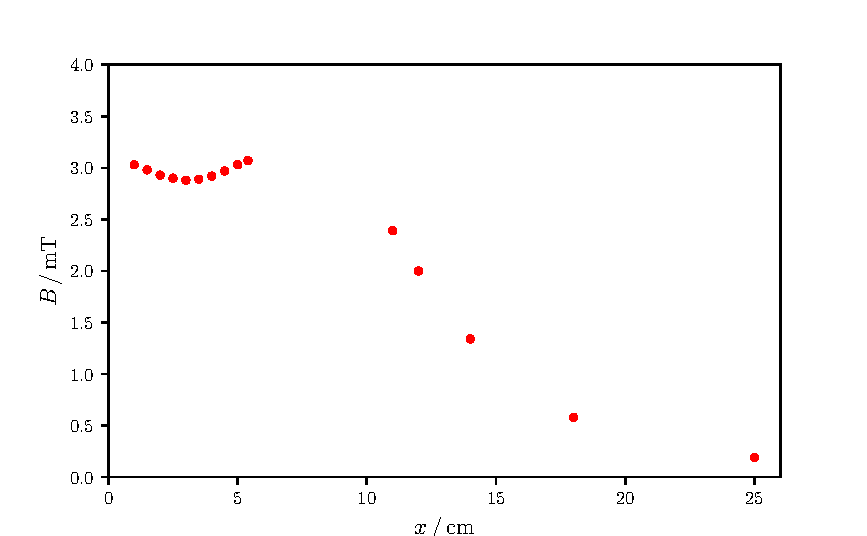
\includegraphics{plot2-1.pdf}
\end{figure}
\begin{figure}
  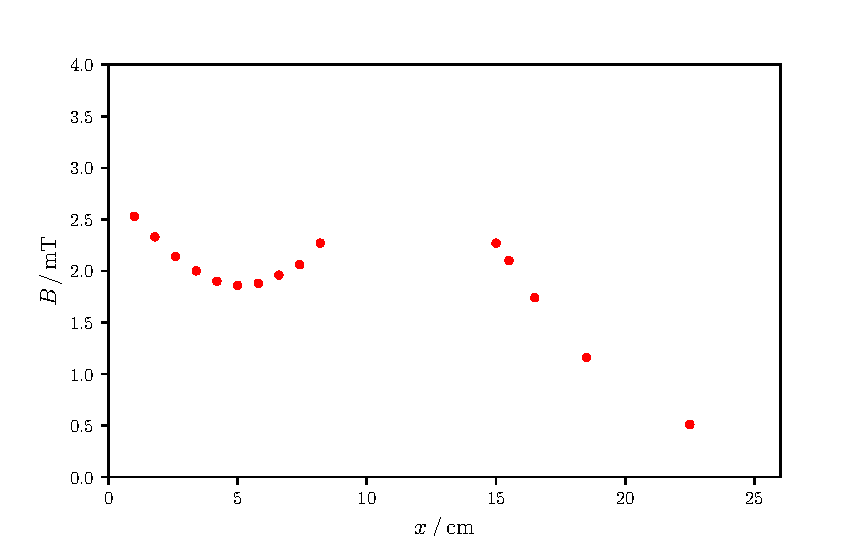
\includegraphics{plot2-2.pdf}
\end{figure}
\begin{figure}
  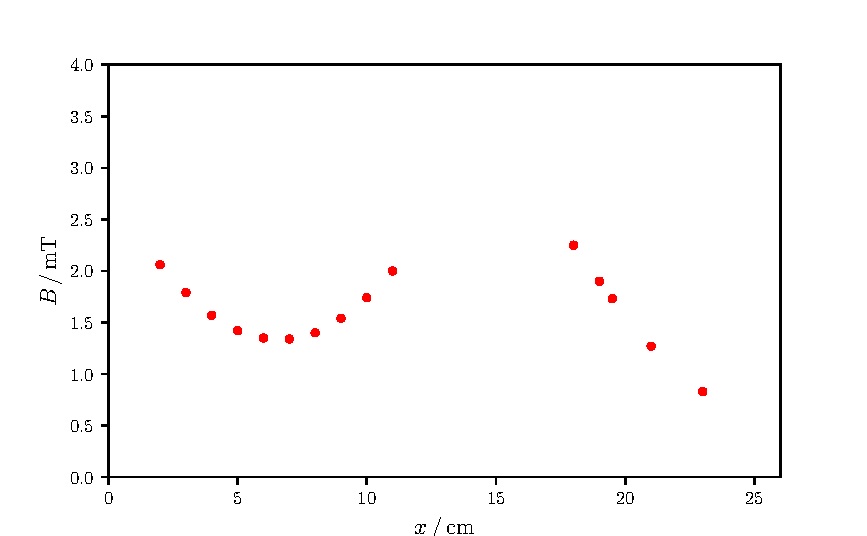
\includegraphics{plot2-3.pdf}
\end{figure}
\begin{figure}
  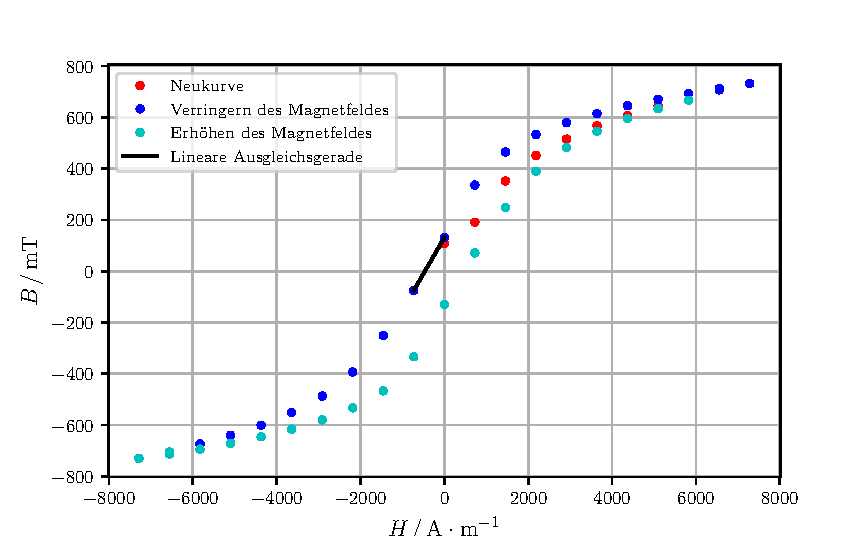
\includegraphics{plot3.pdf}
\end{figure}


